\section{Instrumentos y Equipos}
\begin{itemize}
    \item Transformador monofásico (con datos de placa: tensiones nominales, corrientes nominales, potencia aparente)
    \item Fuente de tensión alterna variable (Variac)
    \item Voltímetros de CA (2 unidades)
    \item Amperímetros de CA (2 unidades)
    \item Vatímetro monofásico
    \item Óhmetro / Multímetro digital
    \item Puente de Wheatstone (opcional, para baja corriente)
    \item Cables de conexión y pinzas
    \item Termómetro (para registrar temperatura ambiente)
    \item Resistencia limitadora de corriente
\end{itemize}

\section{Procedimiento Experimental}

Nota: Antes de iniciar cualquier ensayo, registrar la temperatura ambiente ($T_A$) y las características de placa del transformador (tensiones, corrientes y potencia nominales). Verificar que todos los instrumentos estén calibrados y en el rango adecuado.

\subsection{Medición de Resistencia de los Devanados}

\begin{enumerate}
    \item Identificar los devanados primario (AT) y secundario (BT) del transformador.
    \item Medir la resistencia de cada devanado por el método del voltímetro-amperímetro según el circuito de la Figura~\ref{fig:medicion_resistencia}. Conectar el voltímetro lo más cerca posible al devanado bajo ensayo para evitar incluir la resistencia de los conductores del circuito de corriente.
    \item Ajustar la fuente para que circule una corriente que no exceda el 15~\% de la corriente nominal del devanado.
    \item Tomar al menos cuatro lecturas para cada devanado. Calcular la resistencia como $R = V/I$ para cada lectura y promediar los valores obtenidos.
    \item Desconectar el voltímetro antes de desconectar el transformador para protegerlo de sobretensiones inducidas.
    \item Referir las resistencias medidas a la temperatura de operación ($T_O$) empleando la Ecuación~(3).
\end{enumerate}

\begin{figure}[htbp]
    \centering
    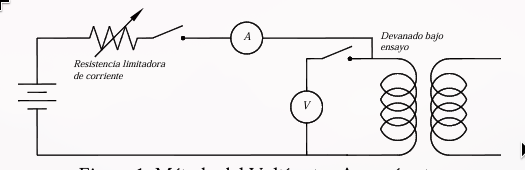
\includegraphics[width=0.7\textwidth]{imagenes/metodo-voltimetro-amperimetro.png}
    \caption{Método del voltímetro-amperímetro para medición de resistencia de devanados.}
    \label{fig:medicion_resistencia}
\end{figure}

\subsection{Medición de la Relación de Transformación}

\begin{enumerate}
    \item Conectar el devanado de AT a la fuente de CA variable a través del Variac. Conectar un voltímetro ($V_{AT}$) en bornes de AT y otro ($V_{BT}$) en bornes de BT.
    \item Aplicar inicialmente no menos del 20~\% de la tensión nominal de AT y realizar cuatro lecturas simultáneas de $V_{AT}$ y $V_{BT}$ incrementando la tensión en pasos del 10~\%.
    \item Intercambiar los voltímetros y repetir la serie de cuatro lecturas con los mismos valores de tensión.
    \item Calcular $a = V_{AT}/V_{BT}$ para cada par de lecturas y promediar ambas series. Cada valor de $a$ no debe diferir de la media en más del 1~\%; en caso contrario, repetir con otros instrumentos.
\end{enumerate}

\subsection{Verificación de Polaridad}

\begin{enumerate}
    \item Conectar el devanado de AT a la fuente de CA. Unir un terminal de AT (H1) con un terminal de BT (X1) mediante un puente.
    \item Conectar un voltímetro ($E_p$) entre los terminales de AT (H1-H2) y otro voltímetro ($E_x$) entre los terminales libres (H2-X2), según la Figura~\ref{fig:polaridad}.
    \item Energizar el circuito con una tensión reducida y registrar ambas lecturas.
    \item Determinar la polaridad:
        \begin{itemize}
            \item Si $E_x > E_p$: polaridad aditiva (H1 y X1 están diagonalmente opuestos).
            \item Si $E_x < E_p$: polaridad sustractiva (H1 y X1 están adyacentes).
        \end{itemize}
\end{enumerate}

\begin{figure}[htbp]
    \centering
    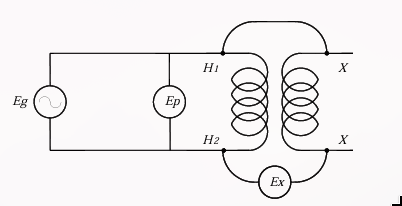
\includegraphics[width=0.6\textwidth]{imagenes/determinacion-de-la-polalidad.png}
    \caption{Circuito para la determinación de la polaridad en un transformador monofásico.}
    \label{fig:polaridad}
\end{figure}

\subsection{Ensayo de Cortocircuito}

\begin{enumerate}
    \item Cortocircuitar el devanado de BT mediante un conductor de baja impedancia.
    \item Conectar el devanado de AT a la fuente a través del Variac, con un vatímetro, un voltímetro y un amperímetro en serie, según las especificaciones de la Figura~\ref{fig:diagrama_cc}.
    \item Aumentar lentamente la tensión hasta que circule por el primario una corriente comprendida entre el 75~\% y el 100~\% de la corriente nominal.
    \item Registrar: tensión de cortocircuito ($V_{cc}$), corriente de cortocircuito ($I_{cc}$) y potencia de cortocircuito ($P_{cc}$).
    \item Corregir la tensión de cortocircuito y las pérdidas a corriente nominal mediante los factores:
        \begin{equation}
            f_{cc} = \frac{I_n}{I_{cc}}, \quad V_{ccc} = V_{cc} \cdot f_{cc}, \quad P_{ccc} = P_{cc} \cdot f_{cc}^2
        \end{equation}
    \item Calcular $Z_{cc}$, $R_{cc}$ y $X_{cc}$ a temperatura ambiente y referirlos a temperatura de operación.
\end{enumerate}

\begin{figure}[htbp]
    \centering
    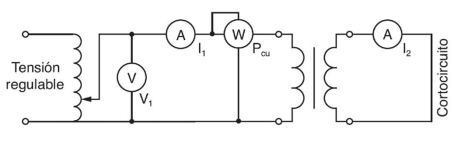
\includegraphics[width=0.7\textwidth]{imagenes/prueba-cortocircuito.png}
    \caption{Diagrama de conexiones para el ensayo de cortocircuito.}
    \label{fig:diagrama_cc}
\end{figure}

\subsection{Ensayo de Vacío}

\begin{enumerate}
    \item Dejar el devanado de AT en circuito abierto.
    \item Conectar el devanado de BT a la fuente a través del Variac, con un vatímetro, un voltímetro y un amperímetro en serie.
    \item Elevar lentamente la tensión desde cero hasta $1,1\,V_n$ sin disminuir en ningún momento. Registrar las lecturas de tensión ($V_0$), corriente ($I_0$) y potencia ($P_0$) en los siguientes puntos: $0,5\,V_n$, $0,8\,V_n$, $1,0\,V_n$ y $1,1\,V_n$.
    \item En caso de requerir un valor menor al nominal, comenzar las mediciones desde cero.
    \item Calcular $R_c$, $X_m$ y el factor de potencia en vacío ($\cos\varphi_0 = P_0 / (V_0 I_0)$) para cada punto de medición.
    \item Trazar las curvas de $I_0$, $P_0$ y $\cos\varphi_0$ en función de la tensión aplicada.
\end{enumerate}

\begin{figure}[H]
    \centering
    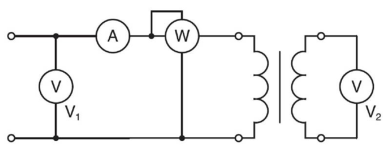
\includegraphics[width=0.7\textwidth]{imagenes/prueba-vacio.png}
    \caption{Diagrama de conexiones para el ensayo de vacío (circuito abierto).}
    \label{fig:diagrama_vacio}
\end{figure}

\newpage
